%------------------------------------------------------------------------
%Editar Diplomado
\hypertarget{cv:modificarCondicion}{\section{Modificar Pre/Postcondición}} \label{sec:modificarCondicion}

	Esta funcionalidad le permitirá modificar la información de una condición previamente registrada con el fin de corregir o actualizar datos del mismo. 

		\subsection{Procedimiento}

			%Pasos de procedimiento
			\begin{enumerate}
	
			\item Oprima el botón \IUEditar{} de algún registro existente de la pantalla \ref{fig:GestionarPrePostcondiciones} ''Gestionar Pre/Postcondiciones''.
	
			\item Se mostrará la pantalla \ref{fig:modificarPrePostcondicion} ''Modificar Pre/Postcondición''.
			
			%Pantalla
			\begin{figure}[htbp!]
				\begin{center}
					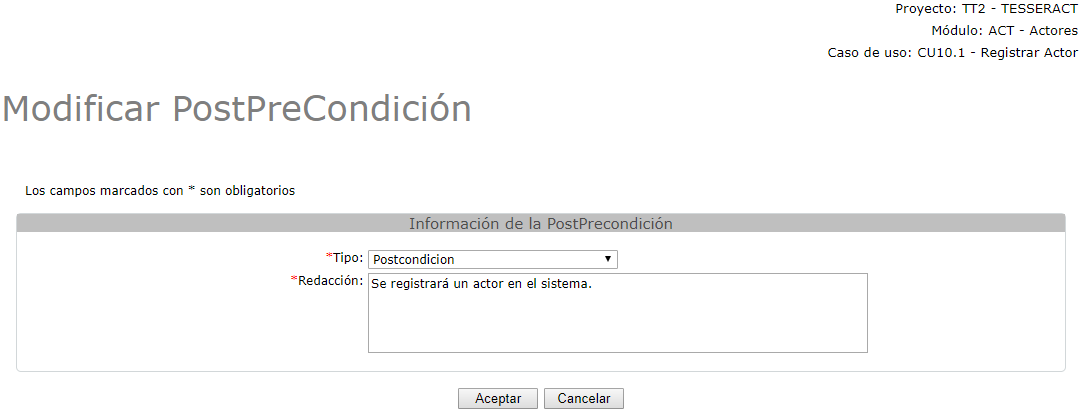
\includegraphics[scale=0.6]{roles/lider/casosUso/precondiciones/pantallas/IU6-1-2-2modificarCondicion}
					\caption{Modificar Pre/Postcondición}
					\label{fig:modificarPrePostcondicion}
				\end{center}
			\end{figure}
		
			\item Modifique los datos solicitados por la pantalla.
						
			\item Oprima el botón \IUAceptar.
			
			\item Se mostrará el mensaje \ref{fig:PrePostModificada} en la pantalla \ref{fig:GestionarPrePostcondiciones} ''Gestionar Pre/Postcondiciones''.
			
			\begin{figure}[htbp!]
				\begin{center}
					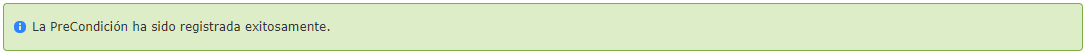
\includegraphics[scale=0.6]{roles/lider/casosUso/precondiciones/pantallas/IU6-1-2-1MSG1}
					\caption{MSG: Condición Actualizada}
					\label{fig:PrePostModificada}
				\end{center}
			\end{figure}
			\end{enumerate}